\chapter{Security Management, Risk and Security Policy}

La gestione della sicurezza è un \textbf{processo formale} per rispondere 
alle seguenti domande:
\begin{itemize}
    \item \textit{quali sono i beni da proteggere?}
    \item \textit{quali sono le possibili minacce?}
    \item \textit{come facciamo a contrastare le minacce?}
\end{itemize}
In ambito IT, la gestione della sicurezza si basa sulla \textbf{valutazione del rischio}.
\begin{enumerate}
    \item bisogna determinare gli obiettivi, le strategie e le politiche 
    di sicurezza dell'organizzazione
    \item eseguire una valutazione del rischio che analizzando le minacce
    determina i rischi risultanti
    \item si devono selezionare dei controlli adeguati per proteggere
    in modo conveniente l'organizzazione
    \item scrivere piani e procedure per attuare i controlli selezionati
    \item monitorare e mantenere l'efficacia dei controlli
    \item rilevare e reagire agli incidenti
\end{enumerate}

La sicurezza è \textbf{lo stato in cui il rischio è inferiore
al massimo rischio accettabile}.


\section{Plan-Do-Check-Act Process Model}
È uno standard (ISO 31000) che descrive un modello per la gestione della sicurezza delle
informazioni, che comprende le seguenti fasi:
\begin{enumerate}
    \item \textbf{Plan:} stabilire politiche, obiettivi e le procedure di sicurezza; si esegue una valutazione del rishcio 
    e si sviluppa un piano di trattamento del rischio
    \item \textbf{Do:} implementare il piano di trattamento del rischio
    \item \textbf{Check:} monitorare e mantenere il piano di trattamento del rischio
    \item \textbf{Act:} mantenere e migliorare la gestione del rischio; risposta ad incidenti o cambiamenti
\end{enumerate}

\begin{figure}[ht]
    \centering
    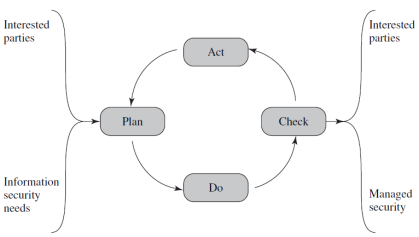
\includegraphics[width=0.75\linewidth]{chapters/images3/plandocheckact.png}
\end{figure}

\section{Rischio}

Il rischio esprime la possibilità che un attacco causi danno ad una organizzazione.

Il rischio viene valutato moltiplicando la \textit{quantità} di danno 
e la probabilità che esso avvenga.

Il rischio può essere valutato utilizzando cinque categorie:
\begin{itemize}
    \item \textbf{Damage potential:} valori dei beni interessati
    \item \textbf{Reproducibility:} difficoltà nel lanciare un attacco; un attacco facile da riprodurre rappresentano un rischio maggiore
    \item \textbf{Exploitability:} sforzo, esperienza e risorse necessarie a lanciare l'attacco
    \item \textbf{Affected users}
    \item \textbf{Discoverability:} \textit{quando verrà rilevato l'attacco?} nel caso peggiore, non saprai mai che il sistema è stato compromesso 
\end{itemize}

\section{Vulnerabilità}
È tutto ciò che può essere sfruttato per recare danno al sistema. Possono
essere classificate in:
\begin{itemize}
    \item \textbf{Critico:} possibile sfruttamento automatico
    \item \textbf{Moderato} sfruttamento mitigato 
    \item \textbf{Basso:} sfruttabilità estremamente difficile
\end{itemize}

\section{Obiettivi della sicurezza}
\begin{itemize}
    \item \textbf{Prevenzione:} impedire agli aggressori di violare la politica di sicurezza
    \item \textbf{Rilevamento:} rileva la violazione della politica di sicurezza da parte dell'attaccante
    \item \textbf{Recupero:} ferma l'attacco, valuta e ripara i danni
\end{itemize}

